%----------------------------------------------------------------------------------------
%	PACKAGES AND OTHER DOCUMENT CONFIGURATIONS
%----------------------------------------------------------------------------------------

\documentclass[10pt,a4paper,oneside]{memoir} % Change font size here (allowable values are 9pt-12pt), change the paper size, specify one or two sided printing and specify whether to show trimming lines

%----------------------------------------------------------------------------------------
%	VARIOUS REQUIRED PACKAGES AND CONFIGURATIONS
%----------------------------------------------------------------------------------------

\usepackage[T1]{fontenc} % Support for more character glyphs
\usepackage[round]{natbib}\citeindextrue % Round brackets around citations, change to square for square brackets
\usepackage{graphicx} % Required to include images
\usepackage{color} % Required for custom colors
\usepackage{amsmath,amssymb,theorem} % Math packages
\usepackage{listings} % Required for including snippets of code
\usepackage{booktabs} % Required for better horizontal rules in tables
\usepackage{xspace} % Provides the ability to use an intelligent space which is used in \institution and \department
\usepackage[printonlyused,withpage]{acronym} % Include a list of acronyms
\usepackage{rotating} % Allows tables and figures to be rotated
\usepackage{hyperref} % Required for links and changing link options
\usepackage{microtype} % Slightly tweak font spacing for aesthetics
\usepackage{float}

\DisemulatePackage{setspace}
\usepackage{setspace} %added in
\doublespacing %added in

\usepackage{booktabs}


% for to do lists, see http://tex.stackexchange.com/questions/9796/how-to-add-todo-notes

\usepackage{xargs}                      % Use more than one optional parameter in a new commands
\usepackage[pdftex,dvipsnames]{xcolor}

\usepackage[colorinlistoftodos,prependcaption,textsize=tiny]{todonotes}
\newcommandx{\unsure}[2][1=]{\todo[linecolor=red,backgroundcolor=red!25,bordercolor=red,#1]{#2}}
\newcommandx{\change}[2][1=]{\todo[linecolor=blue,backgroundcolor=blue!25,bordercolor=blue,#1]{#2}}
\newcommandx{\info}[2][1=]{\todo[linecolor=OliveGreen,backgroundcolor=OliveGreen!25,bordercolor=OliveGreen,#1]{#2}}
\newcommandx{\improvement}[2][1=]{\todo[linecolor=Plum,backgroundcolor=Plum!25,bordercolor=Plum,#1]{#2}}
\newcommandx{\thiswillnotshow}[2][1=]{\todo[disable,#1]{#2}}
%

%\usepackage{amsthm} %for definitions

\hypersetup{colorlinks, breaklinks, linkcolor=black,citecolor=black,filecolor=black,urlcolor=black} % Set up hyperlinks including colors for references, urls and citations

%\definecolor{c64}{rgb}{.063,0,.612} % Example color definition, the color can be used with the \color{name} command

\makeatletter
\renewcommand{\fnum@figure}{\textsc{\figurename~\thefigure}} % Make the "Figure 1.1" text in small caps
\makeatother

%----------------------------------------------------------------------------------------
%	PAGE LAYOUT
%----------------------------------------------------------------------------------------

% The memoir class used in this template contains the ability to set the stock paper size and the trimmed size independently. It also has the ability to show trim lines showing where stock paper should be trimmed to get the final book size. This can all be a bit confusing so please see the memoir class documentation for more information.

% By default, the paper size is a4paper which is 29.7cm × 21cm. To change this, simply change "a4paper" in the \documentclass[a4paper,...]{memoir} command in thesis.tex to another size such as "letterpaper".
% By default, the trimmed size is 24cm x 17cm and trim lines are shown. To remove trim lines, simply remove "showtrims" from the \documentclass[showtrims,...]{memoir} command in thesis.tex. The size of the trimmed content is set with the \settrimmedsize{}{} command below.
% If you wish to remove trims and set the content to fit the paper size (i.e. no trimming at all), all you have to do is remove "showtrims" as above and comment out the \settrimmedsize{}{} command below.

%\setstocksize{24cm}{17cm} % Uncomment to manually set the stock size and override the setting in \documentclass
%\settrimmedsize{24cm}{17cm}{*} % Change the trimmed area size or comment out this line entirely to fit the content to the paper size without trimming
\setlrmarginsandblock{37.125mm}{*}{0.9} % The first bracket specifies the spine margin, the second the edge margin and the third the ratio of the spine to the edge. Only one or two values are required and the remaining one(s) can be a star (*) to specify it is not needed. By default the edge margin is 10% smaller and 
\setulmarginsandblock{37.125mm}{*}{*} % The first bracket specifies the upper margin, the second the lower margin and the third the ratio of the upper to the lower. Only one or two values are required and the remaining one(s) can be a star (*) to specify it is not needed.
\setmarginnotes{17pt}{51pt}{\onelineskip} % The size of marginal notes, the three values in curly brackets are \marginparsep, \marginparwidth and \marginparpush
\setheadfoot{\onelineskip}{2\onelineskip} % Sets the space available for the header and footer
\setheaderspaces{*}{2\onelineskip}{*} % Sets the spacing above and below the header
\setlength{\trimtop}{0pt} % Sets the spacing above the trimmed area, i.e. moved the trimmed area down the page if positive

% Comment the two lines below to reverse the position of the trimmed content on the stock paper, i.e. odd pages will have content on the right side instead of the left and even pages will have content on the left side instead of the right
\setlength{\trimedge}{\stockwidth}
\addtolength{\trimedge}{-\paperwidth}

\checkandfixthelayout % Makes sure your specifications are correct and implements them in the document

%----------------------------------------------------------------------------------------
%	CHAPTER HEADING STYLE
%----------------------------------------------------------------------------------------

\makeatletter
\makechapterstyle{thesis}{
\renewcommand{\chapternamenum}{}
\setlength{\beforechapskip}{0pt}
\setlength{\midchapskip}{0pt}
\setlength{\afterchapskip}{0pt}
\renewcommand{\chapnamefont}{\LARGE}
\renewcommand{\chapnumfont}{\chapnamefont}
\renewcommand{\chaptitlefont}{\chapnamefont}
\renewcommand{\printchapternum}{}
\renewcommand{\afterchapternum}{}
\renewcommand{\printchaptername}{}
\renewcommand{\afterchaptertitle}{\chapnumfont\hfill\thechapter\\\vspace*{-.3cm}\hrulefill\vspace*{6cm}\\}
}
\makeatother

%----------------------------------------------------------------------------------------
%	TABLE OF CONTENTS DEPTH
%----------------------------------------------------------------------------------------

\maxsecnumdepth{subsubsection}
\maxtocdepth{subsection}

%----------------------------------------------------------------------------------------
%	MATH THEOREM DEFINITIONS
%----------------------------------------------------------------------------------------

\theoremstyle{plain}
\newtheorem{thm}{Theorem}[section] % Defines the theorem environment
\newtheorem{prop}[thm]{Proposition} % Defines the proposition environment
\newtheorem{proof}{Proof}[section] % Defines the proof environment
\newtheorem{definition}{Definition}[section] % Defines the definition environment
\newtheorem{example}{Example}[section] % Defines the example environment
\newtheorem{rem}{Remark} % Defines the remark environment
\newtheorem{note}{Note}[section] % Defines the note environment

%----------------------------------------------------------------------------------------
%	CODE SNIPPET CONFIGURATION
%----------------------------------------------------------------------------------------

\lstset{
  basicstyle=\ttfamily\small,
  basewidth=0.55em,
  showstringspaces=false,
  numbers=left,
  numberstyle=\tiny,
  numbersep=2.5pt,
  keywordstyle=\bfseries\ttfamily,
  breaklines=true
}
% Examples of list environments for different programming languages, you will likely need to specify your own
\lstnewenvironment{pseudoc}{\lstset{frame=lines,language=C,mathescape=true}}{}
\lstnewenvironment{logs}{\lstset{frame=lines,basicstyle=\footnotesize\ttfamily,numbers=none}}{}
\lstnewenvironment{cc}{\lstset{frame=lines,language=C}}{}
\lstnewenvironment{c64}{\lstset{backgroundcolor=\color{c64},basewidth=0.65em,basicstyle=\commodoreface\color{c64light},numbers=none,framerule=10pt,rulecolor=\color{c64light},frame=tb,framexbottommargin=30pt}}{}
\lstnewenvironment{html}{\lstset{frame=lines,language=html,numbers=none}}{}
\lstnewenvironment{pseudo}{\lstset{frame=lines,mathescape=true,morekeywords={learn_string_domain, save_model}}}{}
\lstnewenvironment{pseudoctiny}{\lstset{language=C,mathescape=true,basicstyle=\tiny\sffamily}}{}
\lstnewenvironment{cctiny}{\lstset{language=C,basicstyle=\tiny\sffamily}}{}
\lstnewenvironment{pseudotiny}{\lstset{mathescape=true,basicstyle=\tiny\sffamily}}{} % Include the file containing the code defining the structure and style of the document

%------------------------------------------------
% Thesis Information

\title{Development and Testing of an Optimal Cardiometabolic Genetic Risk Score to Predict Coronary Artery Disease Risk} % Thesis title

\author{Christopher B. Cole} % Author name

\date{May 2016} % The date

\newcommand{\institution}{University of Ottawa\xspace} % University/institution name

\newcommand{\department}{Department of Biology\xspace} % Department name

%------------------------------------------------
% Fonts

\renewcommand*{\acffont}[1]{{\normalsize\itshape #1}} % Font style for the acronym text (e.g. Do It Yourself)
\renewcommand*{\acfsfont}[1]{{\normalsize\upshape #1}} % Font style for the acronym in bracket (e.g. (DIY))

%------------------------------------------------
% Hyphenations

\hyphenation{a-no-ma-lous a-no-ma-ly amounts breaches} % Specify custom hyphenation points in words with dashes where you would like hyphenation to occur, or alternatively, don't put any dashes in a word to stop hyphenation altogether

%----------------------------------------------------------------------------------------
%	TITLE PAGE
%----------------------------------------------------------------------------------------

\renewcommand{\maketitlehooka}{
\centering

\includegraphics[width=2.5cm]{Figures/uottawa}\\[.5cm] % Institution logo
\institution\\ % Print institution name
\emph{\department}\\[.2cm] % Print department name
HONOURS B.Sc. BIOMEDICAL SCIENCE, OPTION IN BIOSTATISTICS % Degree or other information
\par
\hrulefill
\vfill}
\renewcommand{\maketitlehookb}{\vfill}
\renewcommand{\maketitlehookc}{
\vfill
\begin{flushleft}
Thesis Supervisor:\\
\textbf{Prof. Ruth McPherson, \tiny{MD, PhD, FACP, FRCPC, FRSC}}\\[.3cm] % Advisor's/supervisor's name
Secondary Thesis Supervisor:\\
\textbf{Dr. Majid Nikpay, \tiny{PhD}} % Doctoral program supervisor's name
\end{flushleft}
\vfill}
\preauthor{\begin{flushright}Honours Dissertation of:\\\bfseries} % Text prior to the author name - right aligned and bold
\postauthor{\end{flushright}} % After the author name, stop right alignment

%----------------------------------------------------------------------------------------

\makeindex % Write an index file

\begin{document}

\begin{titlingpage}
\maketitle % Print the title page
\end{titlingpage}

\frontmatter % Use roman page numbering style (i, ii, iii, iv...) for the pre-content pages




%----------------------------------------------------------------------------------------
%	PREFACE
%----------------------------------------------------------------------------------------

\section*{Preface}

Throughout my undergraduate degree, I have made my fair share of mistakes. In truth, I have made many people's share of mistakes. Like the Rolling Stones, these failures have not always been what I wanted, but oftentimes they were exactly what I needed. This thesis represents the culmination of thousands of lessons taught to me by some truly incredible people.

I would first like to thank Professor Aris-Brosou for taking a chance on a Biomedical Science student first year who knew nothing about programming or statistics, without whom my life would doubtlessly be very different.

I would also like to thank Majid Nikpay, who has been a mentor to me for all of the years I have been researching statistical genetics.

Additionally, I would like to thank all of my friends for the support and motivation they have provided throughout my degree. In particular, I would thank Aaron R. Shifman. He has been a comrade in a lonely field, and a sounding board for my oftentimes less than genius ideas. 

My most heartfelt thanks goes out to my girlfriend of four years, Kennedy Hao. She has motivated me to continue on no matter the obstacle and has proven time and again to be my closest ally, no matter the battle. 

Through any and all obstacles, I have had no further to look for support than to my family. They have helped me through stress, desperation, and have been the only reason I have been able to accomplish the things that I have. Without them, nothing else would be possible.

My final acknowledgment is to my supervisor, Dr. Ruth McPherson. Working with her has been doubtlessly one of the single best decisions of my life. Three years have passed and yet Dr. McPherson continues to help me more in my career and my personal life than I could ever expect of anyone. Truly any success I may claim in the future will be a direct consequence of Dr. McPherson's kindness, generosity, and time.

To everyone, both named and not, I give my most heartfelt thanks. 


\begin{flushright}
\textsc{\theauthor}\\
Ottawa\\
May 2016
\end{flushright}

\cleartoverso % Force a break to an even page



\section*{Dedication}

I, Christopher B. Cole, declare that any and all work presented or implied in this thesis is my own original work and has not been previously presented or submitted for academic publication. 

\cleartoverso % Force a break to an even page


%----------------------------------------------------------------------------------------
%	ABSTRACT
%---------------------------------------------------------------------------------------

\begin{abstract}

\textbf{Background and Rationale}: \ac{CAD} is a major cause of morbidity and mortality globally; much international effort has been expended to detect risk factors, both heritable and environmental. Although there is a well established genetic basis for \ac{CAD}, \acp{GWAS} have identified just 46 significantly associated common loci explaining only a small fraction (~13\%) of the predicted heritability of \ac{CAD}, estimated by twin studies to be between 40 and 60\%. \acp{PRS}, a linear combination of weighted \acp{SNP}, have been successfully used to predict \ac{CAD} with low to moderate accuracy; improvements in the methodology and implementation of these \acp{PRS} are necessary for \ac{PRS} to realize their full clinical potential.

\textbf{Purpose and Specific Objectives}: This study develops and validates two novel methodologies which integrate meta-data from co-morbid conditions to further elucidate the genetic underpinnings of \ac{CAD} while improving phenotype prediction. 

\textbf{Materials and Methods}: Three \acp{PRS} were created using summary information from several large consortia. The first \ac{TRS} model uses the typical procedure for constructing a \ac{PRS}, simply summing over all significant variants weighted by a previously identified risk score. The second risk score incorporates information from several co-morbid traits to re-prioritize the rankings of \acp{SNP} and introduce new variants into the \ac{TRS}. The third creates an optimal score which maximizes the $P$ value of association while minimizing environmental noise. These three scores are constructed, validated in a meta analysis of a population composing 5831 cases and 3832 controls, and compared mathematically in terms of their model fit and their predictive accuracy. 

\textbf{Results}: Both of our novel methodologies proved significantly better than the \ac{TRS} at predicting \ac{CAD}. Additionally, both the \ac{TRS} and the \ac{CMB} score proved superior to 1000 scores composed of equal number of \acp{SNP}, while the \ac{oPRS} did not. We additionally lend evidence to the assertion that genetic risk for high \ac{BMI} is consistent with a model where many small variants act in concert, rather than a few of larger effect size. We demonstrate the superiority of our scores and show them to be important steps forward in the development of better \ac{PRS}.





\end{abstract}

\cleartoverso % Force a break to an even page

%----------------------------------------------------------------------------------------
%	TABLE OF CONTENTS
%----------------------------------------------------------------------------------------

\tableofcontents* % Print the table of contents

\cleartoverso % Force a break to an even page

%----------------------------------------------------------------------------------------
%	LIST OF FIGURES
%----------------------------------------------------------------------------------------

\listoffigures % Print the list of figures

\cleartoverso % Force a break to an even page

%----------------------------------------------------------------------------------------
%	LIST OF TABLES
%----------------------------------------------------------------------------------------

\listoftables % Print the list of tables

\cleartoverso % Force a break to an even page

%----------------------------------------------------------------------------------------
%	ACRONYMS
%----------------------------------------------------------------------------------------

\chapter{List of Acronyms}
\begin{acronym}\addtolength{\itemsep}{-\baselineskip}
  \acro{AIC}{Akaike Information Criterion}
  \acro{CAD}{Coronary Artery Disease}
  \acro{PRS}{Polygenic Risk Score}
  \acro{oPRS}{Optimal Polygenic Risk Score}
  \acro{CARDIOGRAMC4D}{Coronary ARtery DIsease Genome wide Replication and Meta analysis plus The Coronary Artery Disease Genetics}
  \acro{GWAS}{Genome wide Association Study}
  \acro{GLC}{Global Lipids Consortium}
  \acro{GIANT}{The Genetic Investigation of ANthropometric Traits}
  \acro{BMI}{Body Mass Index}
  \acro{MI}{Myocardial Infarction}
  \acro{kb}{kilobase}
  \acro{DNA}{Deoxyribonucleic acid}
  \acro{A}{Adenine}
  \acro{C}{Cytosine}
  \acro{T}{Thymine}
  \acro{G}{Guanine}
  \acro{locus}{specific genetic location}
  \acro{CNV}{copy number variant}
  \acro{InDel}{insertion/deletion}
  \acro{RNA}{ribonucleic acid}
  \acro{SNP}{single nucleotide polymorphism}
  \acro{LD}{linkage disequilibrium}
  \acro{FWER}{family wise error rate}
  \acro{FDR}{false disovery rate}
  \acro{PRDS}{positive regression dependence on subsets}
  \acro{OR}{odds ratio}
  \acro{TG}{triglyceride}
  \acro{HDLc}{high density lipoprotein cholesterol}
  \acro{LDLc}{low density lipoprotein cholesterol}
  \acro{CMB}{cardiometabolic}
  \acro{oCMB}{optimal cardiometabolic}
  \acro{AUC}{area under the curve}
  \acro{OHGS}{Ottawa Heart Genomics Study}
\end{acronym} % Include a List of Acronyms section using acronyms.tex where they are defined

\cleartoverso % Force a break to an even page

%----------------------------------------------------------------------------------------
%	COLOPHON
%----------------------------------------------------------------------------------------

\thispagestyle{empty} % Remove all headers and footers from this page

\vspace*{2em}
\renewcommand{\abstractname}{A note on notation}
\begin{abstract}

Throughout this thesis, the following conventions for notation are used.

\begin{enumerate}
	\item A hat ($\hat{.}$) denotes the estimator of a variable (i.e. $\hat{\beta}$ is the estimator of $\beta$).
	\item Underlining a variable ($\underline{.}$) implies that it is a $n$-vector, or $n \times 1$ dimensional matrix. (i.e. $\underline{Y} = \begin{bmatrix} 1 \\ 0 \\ 1 \end{bmatrix}$ is a $n=3$-vector).
	\item Bolding indicates a matrrix (i.e. $\mathbf{G} = \begin{bmatrix} 1 & \dots & 1 \\ \vdots & \ddots & \vdots \\ 1 & \dots & 1 \end{bmatrix}$)
\end{enumerate}


\end{abstract}
\vfill

%----------------------------------------------------------------------------------------
%	CONTENT CHAPTERS
%----------------------------------------------------------------------------------------

\mainmatter % Begin numeric (1,2,3...) page numbering

\chapterstyle{thesis} % Change the style of the Chapter header to that defined in structure.tex

\pagestyle{Ruled} % Include the chapter/section in the header along with a horizontal rule underneath

\chapter{Introduction}
\label{introduction}

As the efficiency and accuracy of rapid genome sequencing skyrockets, the potential for personalized therapies has made its way from science fiction to scientific reality. Using genetics to understand, diagnose, and eventually to predict illness is not a new idea; in recent years, however, technological ability and scientific understanding have advanced to such a point that researchers may predict risk for several diseases with reasonable confidence. Increasingly, variants in the human genome are being identified as being robustly linked to risk for complex illnesses such as heart disease [\small{cite 9p21}], obesity [\small{cite fto}], and schizophrenia [\small{cite something}]. However, much work remains to be done in order to create tools which may accurately predict individual disease risk from known and unknown genetic risk factors. In this thesis, we propose a novel extension to a well known methodology in order to better characterize disease risk from comorbid conditions using only summary statistics. 

In brief, we present preliminary evidence for the use of \ac{PRS}s in predicting \ac{CAD}. We use recently published summary statistics from a \ac{GWAS} conducted by the \ac{CARDIOGRAMC4D} consortium alongside evidence gathered by the \ac{GLC} and the \ac{GIANT} consortium for lipids and \ac{BMI} \textit{per se}. We use this data alongside previously identified variants to construct first a simplistic \ac{PRS} using only genome wide statistically signficant ($P_{Bonferonni} < 0.05$ or $q_{FDR}$ < 0.05) variants, then expand our search to variants which may not be as robustly linked to phenotype. [Cite storey, BH, and dudbridge]. We use an empirical maximation approach and several strategies of mathematical optimization in order to construct an \ac{oPRS}, then devise a novel technique for integrating information from co-morbid \ac{oPRS} diseases in order to better predict \ac{CAD} in four cohorts comprising approximately $n=12,000$ individuals

\section{Genetics of Coronary Artery Disease}

\ac{CAD} occurs when the major blood vessels supplying the heart become diseased or damaged, often leading to severe complications such as \ac{MI} and death. [cite review articles] \ac{CAD} is known to be a complex genetic disease with heritability estimated by twin studies between 40 and 60\%. [mcPherson 2016, twin studies paper] Several important variants have been identified which have been shown to robustly increase risk to \ac{CAD} by altering lipid transporting pathways, structural collagen bodies, and others factors. [cite]


\begin{figure}[h]
\caption{Progression of the formation of plaque causing \ac{CAD}. Adapted from Gretch 2003.}
\centering
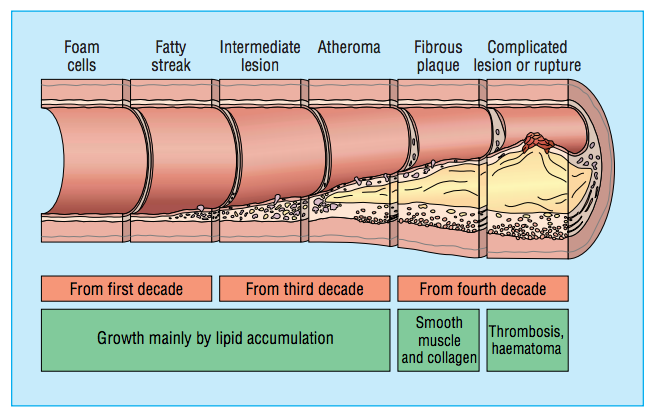
\includegraphics[width=0.8\textwidth]{Figures/cad.png}
\end{figure}

With heart disease and stroke the leading cause of prescription drug use in Canada as well as one of the leading causes of death and hospitalization [cite herat and stroke], the need to better understand, diagnose, and prevent this deadly disease is apparent.  In order to better understand the need for improved statistical methodologies, it is important to understand the large body of previous attempts to characterize the genetic determinants of \ac{CAD}

Despite some promising beginnings, initial attempts to understand and explain \ac{CAD} through genetics were largely unsuccessful.[CITE] The first variant to be successfully and robustly linked to risk for \ac{CAD} was the 9p21.3 locus. Discovered by a team of researchers at the University of Ottawa Heart institute, the allele consists of a 58 \ac{kb} region on chromosome 9 which was shown to be associated with \ac{CAD} in a population of 23,000 Caucasian individuals. (\cite{McPherson2016})

\begin{figure}[h]
\caption{Fine mapping of the genomic interval on chromosome 9 associated with Coronary Heart Disease. Adapted from Mcpherson et al 2006}
\centering
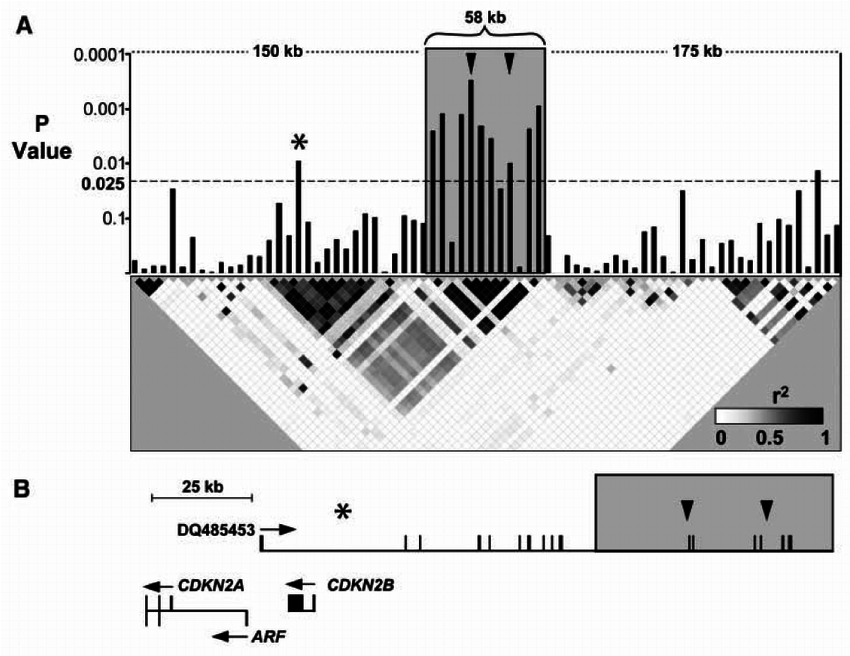
\includegraphics[width=0.8\textwidth]{Figures/9p21.png}
\end{figure}

This initial success began the era of the \ac{GWAS}, explained in more detail in section \ref{gwas}.  Researchers across the globe began frantically searching for more loci with the hope of understanding and predicting complex disease; in that goal, the \ac{GWAS} has failed. (\cite{Visscher2012}) A number of important genetic markers for \ac{CAD} have been discovered, but often in small familial cases or with very low effect sizes. [Cite] As the dust settles and the low hanging fruit have been picked, common variants have been shown to explain approximately 28\% of the heritablity of \ac{CAD} [cite majid], yet a large portion remains to be accounted for. This has become known as the problem of ``missing heritabillity'' of complex disease; common genetic variants explain a relatively small portion of the total estimated heritability of a disease, therefore researchers must resort to ever more obscure and complex methods to attempt to explain the complex interactions between genetic elements in the human genome. [cite review paper] From pathway analysis to partitioned heritability to all kinds of arcane statistical procedures, researchers from across the globe have tried their hardest to shrink this gap between our knowledge and accurate prediction and understanding of complex disease. To this end, we develop our own methodology incorporating multiple sources of information for the more accurate prediction of clinical end points. 

\section{Genome Wide Association Studies} \label{gwas}

In order to properly introduce the model, however, the basic underpinnings must be explored and explained. Genome wide association studies seek to indetify associations between individual genotypes and disease phenotypes in a hypothesis free manner. In this section, the statistical model required to understand \ac{GWAS} is presented and explored.

\subsection{Primer on Genetics}

\ac{DNA} is a double helical molecule which encodes the genetic blueprints for the construction of proteins and other materials that make up every known living organism. \ac{DNA} is composed of three parts: a negatively charged phosphate group, a five carbon sugar \textit{deoxyribose}, and (usually) one of four nitrogen bases. It is these bases, \ac{A}, \ac{C}, \ac{T}, and \ac{G} and their combinations which are under investigation in a \ac{GWAS}. The specific combinations of these four bases in a \ac{locus} determine the product produced by the \ac{DNA}, and even a small change in this order can have large ramifications on the overall health, survival, and proper function of the organism. 

\subsection{Sequencing}

DNA sequencing is the process of ascertaining a particular individual's genotype by means of chemical identification of the bases present at predefined sites. [cite] These sites, whether they be a change in a single base called a \ac{SNP}, a variation in the number of tandem repeats of a small sequence named a \ac{CNV} or an \ac{InDel} of a sequence, may alter amino acid sequence, affect regulatory regions, or impact regulatory \ac{RNA} sequences.

\begin{definition}[Allele]
A specific form or subtype of a genetic locus. This could be one or more individual variations or a combination therof. 
\end{definition}

\begin{rem}
Allele frequency is the frequency at which a particular allele occurs in the population. I.e. for locus $A$ having $n$ different alleles, the true population allele frequency of allele $freq A_m \equiv \frac{A_m}{ \sum^n_{i=1} A_i}$, which is estimated in a sample population with a biased ratio estimator $freq \hat{A}_m \equiv \frac{\hat{A}_m}{ \sum^n_{i=1} \hat{A}_i}$  
\end{rem}

\subsection{Statistical Definition}

Consider a simple case control population where 1 defines case and 0 defines control. Define $\underline{\mathbf{Y}}$ as an $n$-vector where $n$ denotes the number of individuals in a population and $\underline{\mathbf{Y}}_i$ gives the individual's diesease staet. Additionally define $G$ as an $m \times n$ matrix where $m$ is the number of informative genotypic sites available with $\mathbf{G}_{ij}$ being the ``state'' (allele number) present at site $j, 1 \leq i \leq m, i \in \mathbb{Z}^+$ in individual $i, 1 \leq i \leq n, i \in \mathbb{Z}^+$.

$$ \begin{aligned} &\mathbf{\underline{Y}} &= \begin{bmatrix} Y_1 \\ \vdots \\ Y_n \end{bmatrix} \, \, \, \, \, \, \, \,\, \, \, \,\, \, \, \, \, \, \, \, \, \, \, \,\, \, \, \,\, \, \, \, &  \mathbf{G} &= \begin{bmatrix} G_{1,1} & \dots & G_{1, n} \\ \vdots & \ddots & \vdots \\ G_{m, 1} & \dots & G_{m, n} \end{bmatrix} \end{aligned} $$

In an additive genetic model, we define the phenotype $\underline{\mathbf{Y}}$ as a linear combination of $\mathbf{G}$ weighted by a vector of $\underline{\mathbf{\beta}}$ coefficicent vectors estimated by regression analysis and $\underline{\mathbf{\epsilon}}$ vector of errors. Express $\underline{\mathbf{Y}}$ such that

$$ \underline{\mathbf{Y}} = \underline{\mathbf{\beta}}' \mathbf{G} + \underline{\mathbf{\epsilon}} = \left( \sum^m_{i=1} \beta_i \mathbf{G}_{i, n} + \epsilon_n \right)' $$

$\underline{\mathbf{\beta}}$ and $\underline{\mathbf{\epsilon}}$ are approximated optimally by $\underline{\hat{\beta}}$ and $\underline{\hat{E}}$ in practice.

The purpose of a \ac{GWAS} is not only to estimate these genetic effects $\underline{\mathbf{\beta}}$ by $\underline{\hat{\beta}}$ but also to estimate their significance of association with phenotype vector $\underline{\mathbf{Y}}$ through a $\chi^2$ test and corresponding test statistic $m$-vector $\hat{\chi}^2$. The degrees of freedom of this test statistic will vary between methods and models, and so will be left as futher reading. 

\ac{GWAS} commonly estimate these effects through linear regression. The disease state (or disease level, should it be a continuous variable) is used as the response variable, while the main dependent variable is usually the number of minor alleles (0, 1, or 2) present.  The $\beta$ coefficient (for continous disease state) or \ac{OR}, therefore represents the average increase (for the continuous case) or the \ac{OR} per additional risk allele present. 


\begin{rem} This description assumes an additive genetic model, which states that the effect of possessing one minor allele is exactly the same as half the effect of having two risk alleles. Additional genetic models include the dominant scheme, where the effect of having two minor alleles is the same as having one minor allele, the recessive scheme where only the case of two minor alleles impacts the phenotype, and the general genetic model, where the effect of one allele is $a \times$ the effect of two alleles, $a \in [0,1]$. \end{rem}
 
By approximating $\underline{\chi^2}$ with $\hat{\underline{\chi^2}}$ and computing the corresponding $P$ values, reserchers are able to identify and quantify the effects of variants significantly ($P < 0.05$) associated with the phenotype. These results can be summarized in a Manhattan plot, named after the city of Manhattan with it's high rise buildings towering over the scenery. The $x$ axis of this plot is the genomic location (usually coloured by chromosome number) while the $y$ axis is the $\log_{10}$ of the $P$ value of association derived from $\hat{\underline{\chi^2}}$. 


\begin{figure}[H]
\caption{Example of a Manhattan plot from a \ac{GWAS} for \ac{CAD} performed by Shunkert et al. 2011}
\centering
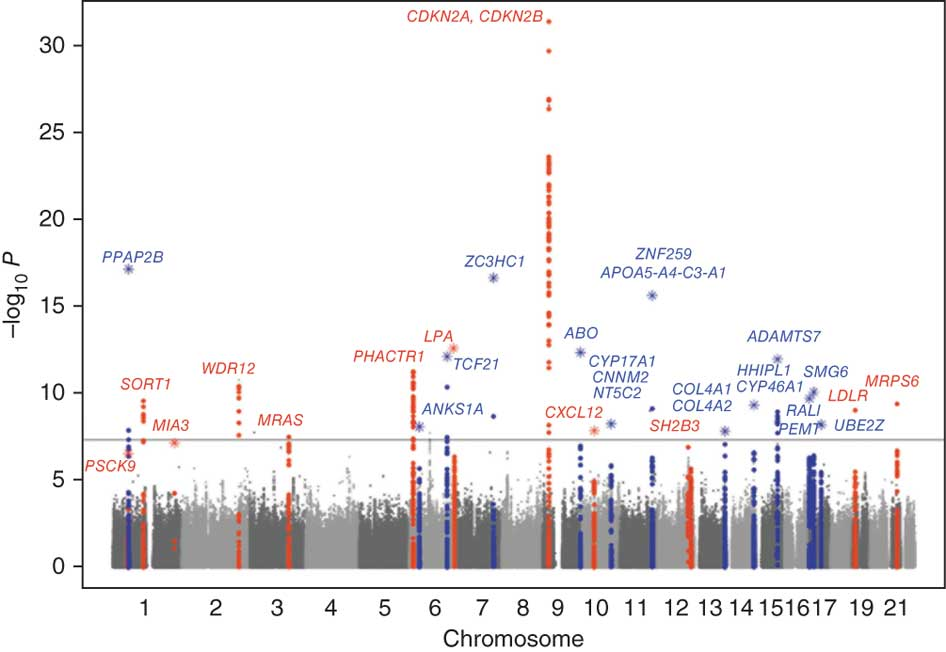
\includegraphics[width=0.5\textwidth]{Figures/man_ex.jpg}
\end{figure}

\subsection{Multiple Comparisson Problem}

In such a set up, where $m$ may be in the millions and the threshold of significance is set to $P = \alpha = 0.05$, we encounter a canonical issue in statistical inference. Recall that $P$ is the probability of observing a $\chi^2$ statistic as large or larger than a specific $\chi^2_m$ assuming $H_0$ of no association is correct and $\alpha$ is the threshold at which a significant effect is declared. Table \ref{hyptest} introduces relevant notation for this section. 


\begin{table}[H]
\centering
\caption{Notation relating to hypothesis testing. Adapted from \cite{Sun2006}}
\label{hyptest}
\begin{tabular*}{.8\linewidth}{@{}llll@{}}
\toprule
                                  & \textbf{True $H_0$} & \textbf{True $H_1$} & \textbf{Total} \\ \midrule
\textbf{Declared significant}     & $V$                 & $S$                 & $R$            \\
\textbf{Declared non-significant} & $U$                 & $T$                 & $m - R$        \\
\textbf{Total}                    & $m_0$               & $m - m_0$           & $m$            \\ \bottomrule
\end{tabular*}
\end{table}


For the sake of description, we define $M$ as the number of \textit{independant} variants (that is, the effective number of variants which are not in \ac{LD} for a given $R^2$ or $D'$ threshold) for sake of description. Thus, $M$ tests and corresponding $M$-vector of $P$ values $\underline{\mathbf{P}}$ is constructed. Because in any statistical test, assuming that $H_0$ is true, there is $\alpha$ chance of falsely rejecting $H_0$ (type I error), by increasing the number of simultaneous tests conducted, the probability of falsely rejecting $H_0$ compounds exponentially as a function of the number of independent test conducted. That is, the conditional probability of falsely rejecting $H_0$ for all $M$ tests may be written as 

$$ Pr(P \leq \alpha \, | \, H_0) = 1-(1 - \alpha)^M $$

This may equivalently be described as the probability of making at least one false positive in $M$ tests. This may alternatively be notated 

$$ Pr(V \geq 1) = 1-(1 - \alpha)^M $$

Speaking asymptotically, $\lim_{M \to \infty} 1-(1 - \alpha)^M = 1$ and false positves are guarenteed. It is against this backdrop that we recall in any relevant genetic context, $M$ is large, and false positives are almost guarenteed.

There exist several ways to correct for this issue, chief among them is the widely adopted Bonferroni correction. Put simply, Bonferroni correction adjusts testing such that $Pr(V \geq 1) = \alpha$ rather than $1-(1 - \alpha)^M$. It does so by rejecting all tests $p_i \in \underline{\mathbf{P}} | i \in 1 \dots M, i \in \mathbb{Z}^+$ such that

$$ p_i \leq \frac{\alpha}{M} $$


The proof is not complex, but shall not be presented here for the sake of brevity. [cite bf]  This adjustment (for $Pr(V \geq 1)$) is defined as control of the \ac{FWER}. This approach does not make any assumptions about the internal dependency strucutre of the tests, and as such, is conservative in the case of all categories of dependency. This is often undesired, as typically researchers will not prune their \ac{GWAS} data to only independant variants. A more commonly accepted procedure, controlling the \ac{FDR} rather than the \ac{FWER} adjusts $\underline{\mathbf{P}}$ such that the proportion of false disoveries in all discoveries is controlled at $\alpha$: 

$$ FDR \equiv E \left[ \frac{V}{R} \right] = \alpha $$

This approach has the benefit of being adaptable and more powerful in circumstances of some forms of dependency (most notably \ac{PRDS} which is common scenario) and is most often applicable to \ac{GWAS} where researchers are more willing to find more true positives at the cost of a fraction of false positives.

Therefore, in summation, \ac{GWAS} is a statistical investigation which estimates several parameters given certain assumptions. Concepts presented in this section will be important background knowledge for the following sections, as most of our model builds off of these premeses. 

\section{Polygenic Prediction of Complex Disease}

Refering to the defintions proposed in the previous section and recalling that in a general additive model, a phenotype vector $\underline{\mathbf{Y}}$ may be expressed as a linear combination of the $\underline{\beta}$ weighted genetic $n \times m$-matrix $\mathbf{G}$ and $\underline{\epsilon}$ following a standard normal $N(0, 1)$ distrbution: 

$$ \underline{\mathbf{Y}} = \underline{\beta}' \mathbf{G} + \underline{\epsilon} $$

It has been previously proposed to combine genetic variants in order to crease a score $S$ which encompases estimated genetic effects in order to predict the phenotype vector $\underline{\mathbf{Y}}$. Define $S$ for individual $n$:

$$ S_n = \sum^m_{i=1} \beta_i G_{ni} $$

Note that in practice, our true statistics must be estimated. The logical estimator of $\underline{\beta}$ is the ordinary least squares regression estimator $\hat{\beta}$. There are other estimators, but the remainder of this section assumes this estimator. Our score is therefore described as:

\begin{equation} 
\label{score}
\begin{aligned}
\hat{S}_n = \sum^m_{i=1} \hat{\beta}_i G_{ni} 
\end{aligned}
\end{equation}

This score has several important properties which will be exploited in the below analysis. Note that in practice, $\underline{\beta}$

Notably, the non-centrality parameter of the $\chi^2$ test for association between $\hat{S}$ and $\underline{Y}$ in the test population, assuming that $\hat{\beta}$ has been estimated in a training population of size $n_1$ and tested in a test population of size $n_2$, is given by:

$$ \lambda = \frac{n_2 R^2_{\hat{S}, Y}}{1 - R^2_{\hat{S}, Y}} $$

Where $R^2_{\hat{S}, Y}$ is the percent explained variance of the phenotype $Y$ with the estimated score $\hat{S}$. 

Additionally, note that $E[\hat{S}] = 0$ and the second moment in a particular individual is given by

$$ \begin{aligned} Var(\hat{S}) &= \sum^m_{i=1} Var(\hat{\beta}_{il}, G_{i}) \\ &= \sum^m_{i=1} \hat{\beta}_{i} \\ &\approx m Var(\hat{\beta}_{i}) \end{aligned} $$

These mathematical properties become important later. These identities have been adapted from \cite{Dudbridge2013}.

\section{Optimal Polygenic Risk Scores}
\label{oPRS}

Frequently, not all $m$ variants are used in the construction of the \ac{PRS} though. Typically, researchers will type the top $m | P_m \leq \alpha_{adj}$ where $\alpha_{adj}$ denotes the shifted acceptance threshold after multiple testing correction. We denote these variants as $m_{P \leq T}$ where $T$ is the $P$ value threshold. 

Though these variants have the highest probability of being truly associated with the phenotype, constructing a score with this few \ac{SNP}s misses the many small and insignificant effects hidden in marginally significant and insignificant hits. Thus, \cite{Euesden2014} have developed a method to find the best-fit \ac{PRS}, that is, the PRS which maximizes genomic signal while minizing noise as in \ref{pt}. We denote this as the \ac{oPRS}. 

\begin{figure}[h]
\label{pt}
\caption{\ac{oPRS} plot for schizophrenia predicting major depresive disorder status. Adapted from \cite{Euesden2014}}
\centering
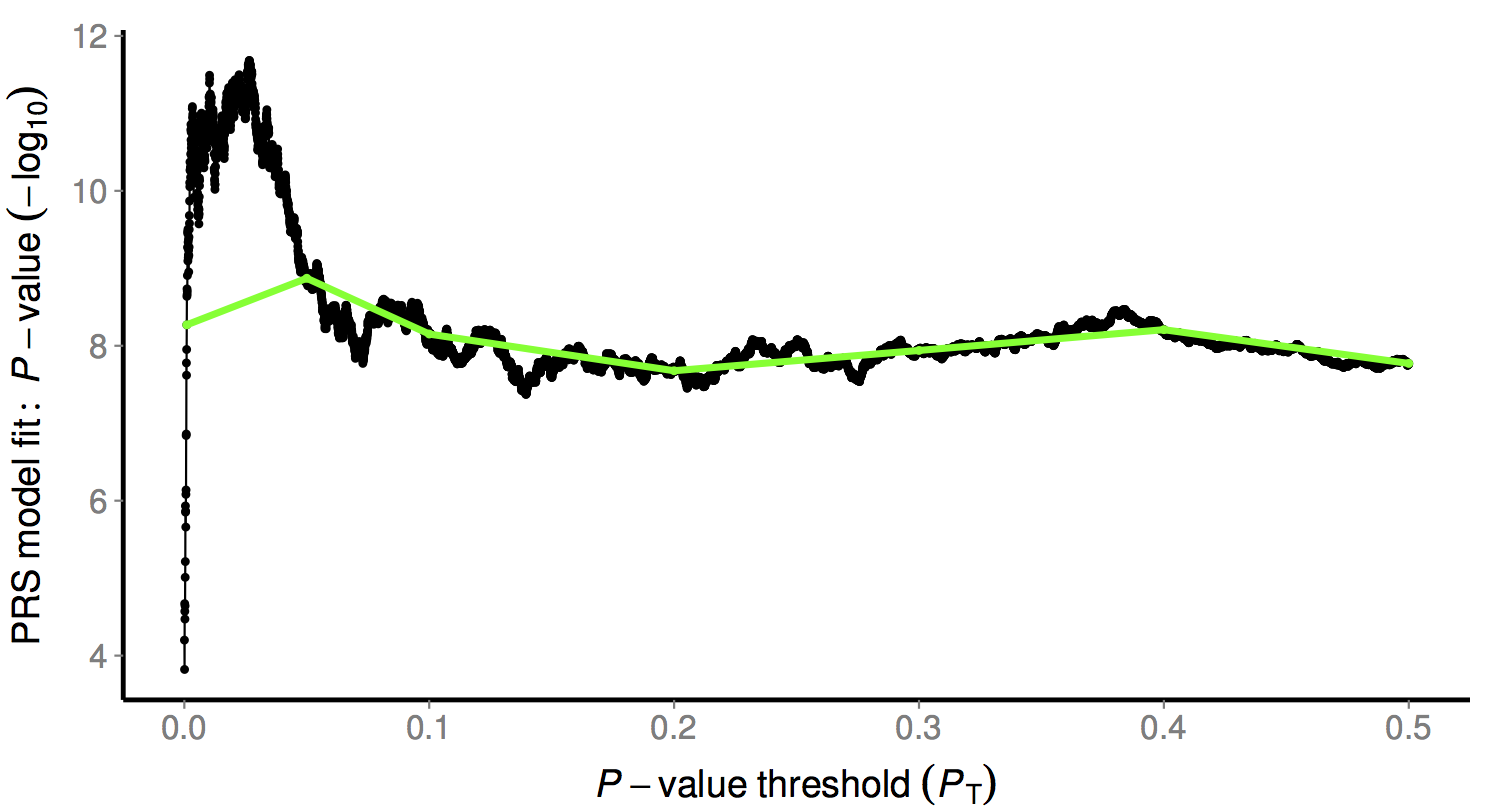
\includegraphics[width=0.8\textwidth]{Figures/pt.png}
\end{figure}

On a high level, this score involves iterating through a list of $P$ value thresholds $T$, constructing a score using all $m_{P < T}$ and selecting either the smallest $P$ value of association between $\hat{S}$ and $\underline{\mathbf{Y}}$ or the highest $R^2_{\hat{S}, Y}$ to move in the analysis. 

More formally, we fix individual $n$ and construct a vector of estimated scores $\underline{\hat{S}}$ with length $n_T$ equal to the number of attempted $P$ value thresholds. 

$$ \begin{aligned} \underline{\hat{S}} &\equiv \begin{bmatrix} \hat{S}_{T_1} \\ \vdots \\ \hat{S}_{n_T} \end{bmatrix} &&&&& \hat{S}_T &= \sum^{m_{P \leq T}}_{i=1} \hat{\beta}_i G_{ni} \end{aligned}$$

Note, however, that when we build a score at each threshold for each individual, an $n \times T$ matrix is constructed, where $n$ is the number of individuals and $T$ is the number of thresholds. The entries are the estiamted score $\hat{S}_{nT}$ for individual $n$ at threshold $T$:

\begin{equation} 
\label{score_matrix}
\begin{aligned}
\mathbf{\hat{S}} = \begin{bmatrix} \hat{S}_{1,1} & \dots & \hat{S}_{1, T} \\ \vdots & \ddots & \vdots \\ \hat{S}_{n, 1} & \dots & \hat{S}_{n, T} \end{bmatrix}
\end{aligned}
\end{equation}

It is from the matrix described in \ref{score_matrix} that the rest of our model will be built.

\begin{figure}[h]
\label{pi0}
\caption{Expected $-\log_{10} (P)$ value of linear regression estimate as a function of $P$-value threshold for selecting markers into Polygenic score. Note that $\pi_0$ refers to the proportion of \textit{true null} markers, that is, markers which have no effect on phenotype. (\cite{Dudbridge2013})}
\centering
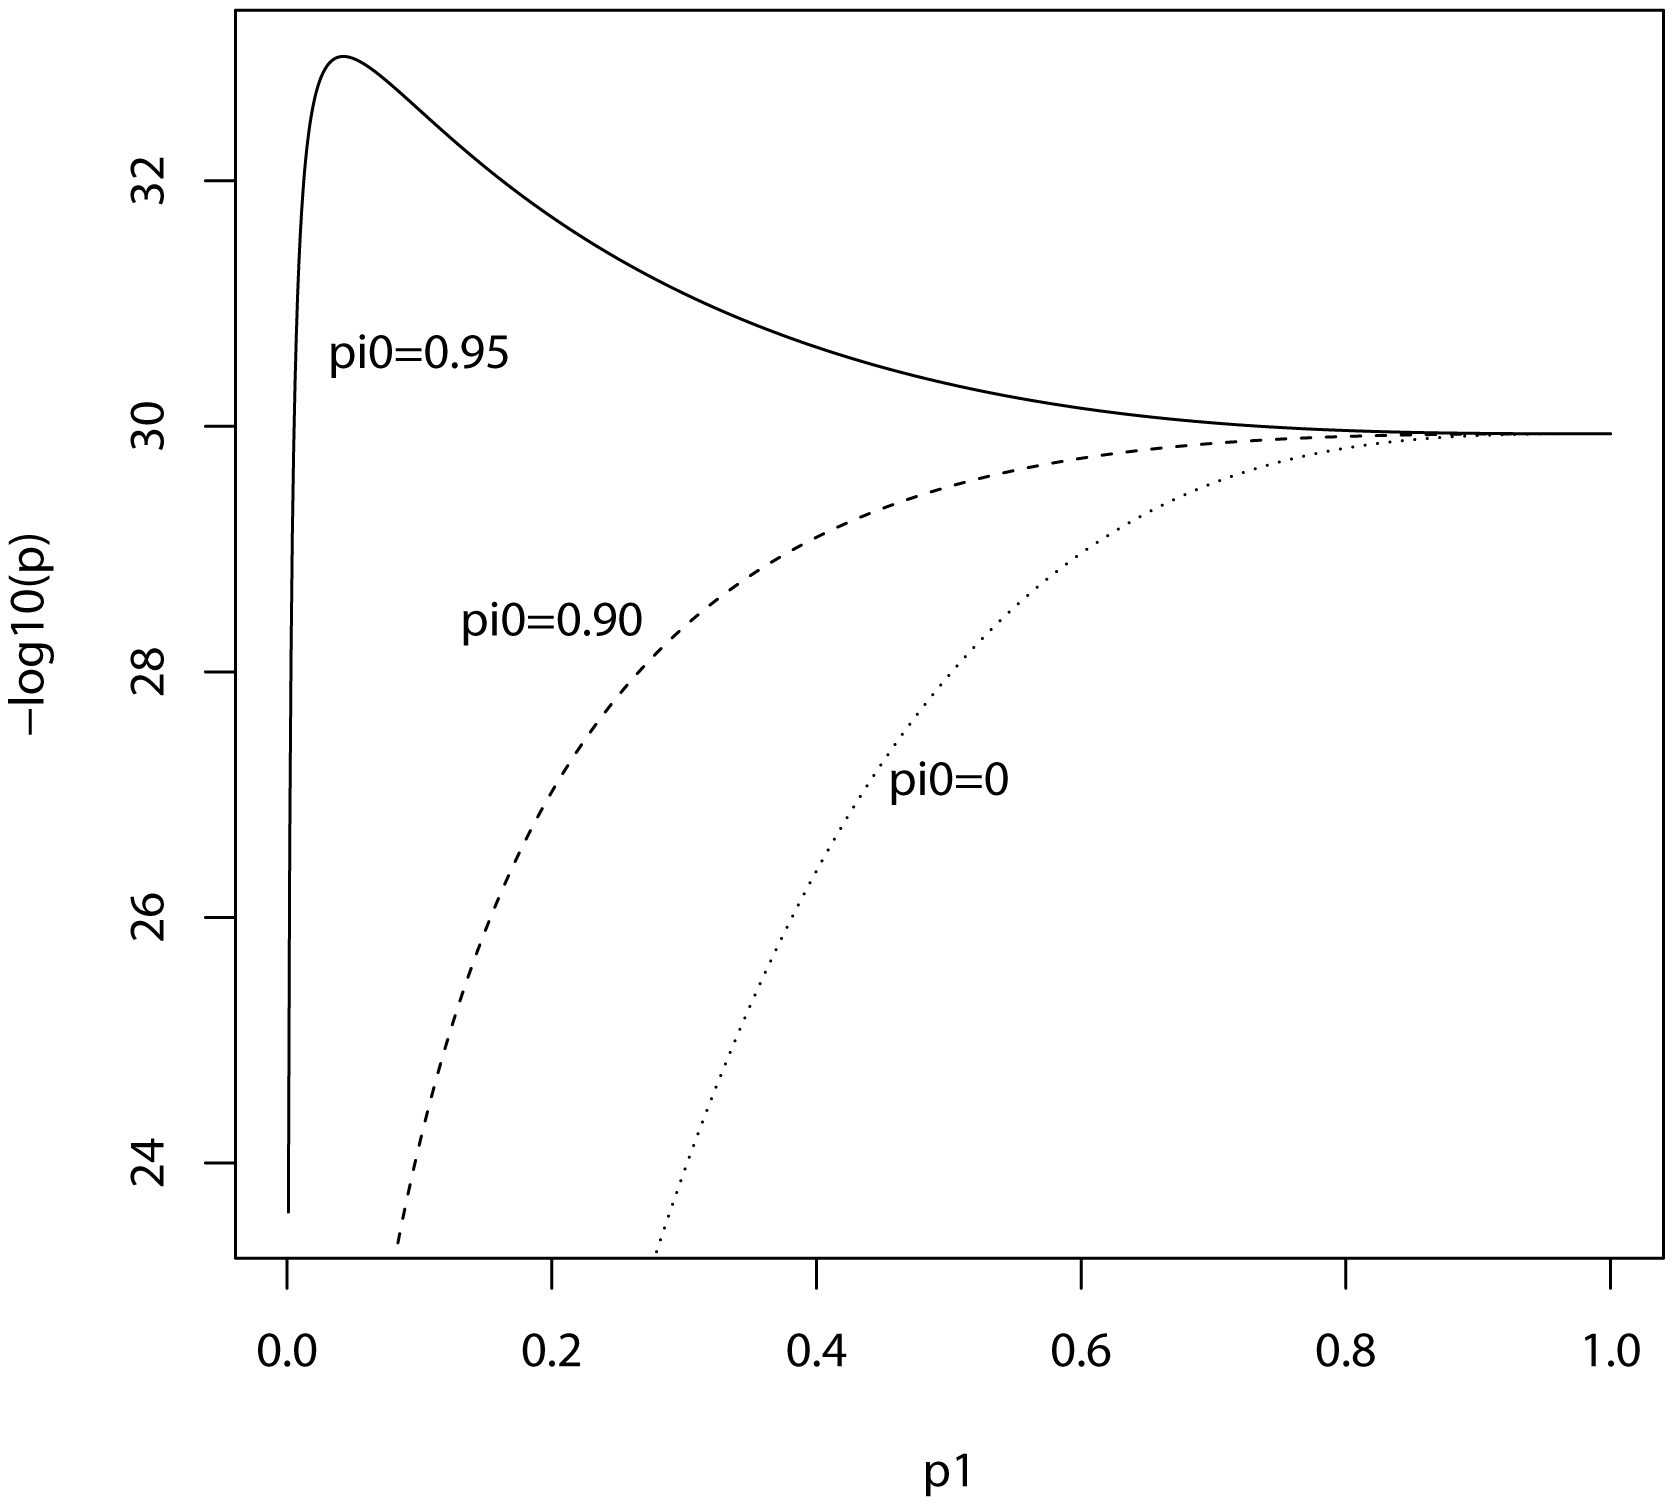
\includegraphics[width=0.8\textwidth]{Figures/pi0.png}
\end{figure}

\begin{rem}
Though it is always possible to construct an optimal score, only in certain circumstances is the $P$ value threshold $P_T < 1$, depending on the internal structure of the disease under question. At different heritability levels, a disease may only have an optimal score with $P_T =1$, as described in Figure \ref{pi0}.
\end{rem} 

\section{Specific Aims}

This study plans to address the following issues:

\begin{enumerate}
	\item Characterize and evaluate the predictive accuracy of the traditional risk score (\ac{TRS}). Evaluate summary statistics for regression models and perform a meta analysis across cohorts to estimate an overall effect for the model. 
	\item Propose two novel applications of \ac{PRS} to better predict \ac{CAD}. Develop these methods mathematically, validate them in test sets, and compare their performance to the traditional risk score.
	\item Perform an exploratory analysis on secondary data to further evaluate the effectiveness of risk scores in predicting \ac{CAD}.
	\item Discuss possible theoretical ramifications of findings, applications, and further research.
\end{enumerate}
 % Include the introduction chapter
\chapter{Methods}
\label{methods}

Building on the previously introduced notation, we introduce the present study.

\section{Study Population}

\subsection{Population Descriptions}

\section{Genotyping and Imputation}


\section{Training Populations}

\subsection{GIANT Consortium}

\subsection{Global Lipids Consortium}

\section{Polygenic Prediction of CAD}

\subsection{Traditional Risk Score}

\subsection{Cardiometabolic Risk Score}

\subsection{Optimal Cardiometabolic Risk Score}

 % Include the first content chapter
\chapter{Results}
\let\cleardoublepage\clearpage 

General characteristics of the study population are displayed in Table \ref{pop}.
\tabularnewline
\tabularnewline

\begin{table}[bp]
\centering
\begin{tabular}{llllll}
\hline
                   & All Participants &  & Cases       &  & Controls    \\ \hline
n                  & 9663             &  & 5831        &  & 3832        \\
Age$^1$ (years)       & 62.8 $\pm$ 12.3      &  & 56.2 $\pm$ 10.1 &  & 73.0 $\pm$ 7.4  \\
Smoke Current (\%) & 29.6             &  & 36          &  & 20          \\
Male (\%)          & 65.3             &  & 76.7        &  & 47.9        \\
Obese $^2$ (\%)       & 29               &  & 35.1        &  & 19.7        \\
BMI (kg/$m^2$)        & 28.1 $\pm$ 5.3       &  & 28.9 $\pm$ 5.3  &  & 26.7 $\pm$ 4.9  \\
TG $^3$ (mmol/L)      & 1.46 $\pm$ 1.47      &  & 1.66 $\pm$ 1.70 &  & 1.18 $\pm$ 0.99 \\
HDLc$^3$ (mmol/L)     & 1.27 $\pm$ 0.44      &  & 1.13 $\pm$ 0.39 &  & 1.46 $\pm$ 0.44 \\
LDLc$^3$ (mmol/L)     & 3.29 $\pm$ 1.08      &  & 3.18 $\pm$ 1.17 &  & 3.43 $\pm$ 0.93 \\ \hline
\end{tabular}
\caption[General Population descriptions.]{General Population description. All values are expressed as mean $\pm$ one standard deviation unless otherwise noted. $^1$  Age represents age at consent for controls and age at diagnosis for cases
 $^2$ Obesity is defined as having a BMI of greater or equal to 30 kg/m2 at time of collection $^3$T G (triglyceride), LDLc (low density lipoprotein cholesterol), HDLc (high density lipoprotein cholesterol).}
\label{pop}
\end{table}


\section{Traditional Risk Score}

The traditional risk score was significantly ($P < 2.2 \times 10^{16}$) associated with case/control status in all cohorts when adjusted for principal components to control for population stratification. \citep{Price2006,Zhang2013}. On average, scores between cases and control differed by $5.06 \times 10^{-4} \pm 1.73 \times 10^{-4}$. $\hat{S}_{TRS}$ predicted CAD status better than chance in all cohorts. Area under the receiver operator characteristic curve was calculated for each model and meta-analyzed. The resulting AUC $\pm$ 95\% confidence intervals are displayed in Figure \ref{trs_meta}.

\begin{figure}[h]
\label{trs_meta}
\centering
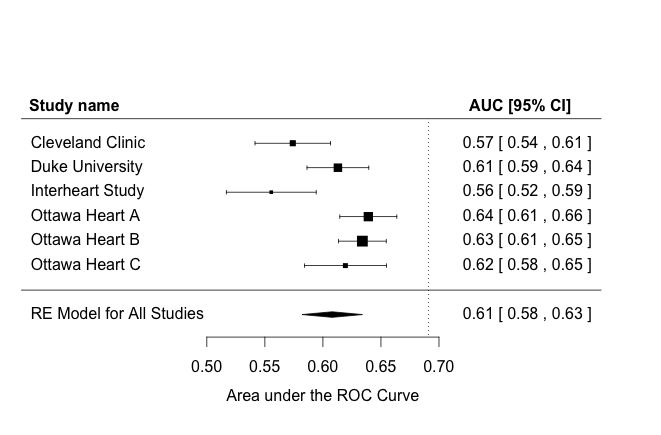
\includegraphics[width=0.8\textwidth]{Figures/trs_meta.png}
\caption[Random effects meta analysis of AUC ROC from six cohorts.]{\textbf{Random effects meta analysis of AUC ROC from six cohorts.} Logistic regression models were constructed with $\hat{S}_{TRS}$ and the first two principal components adjusting for population stratification were used to predict \ac{CAD}. Various thresholds for false positives and true positives were used to construct \ac{ROC} curves. Area under these curves were estimated along with error. The associated effects were analyzed assuming cohorts were random effects and an overall effect was derived.}
\end{figure}

Logistic regression was used to predict observations following the model. Summary statistics from the models employed are displayed in Table \ref{trs}

$$ CAD = X_0 + \hat{\beta}_1 \hat{S}_{TRS} + \hat{\beta}_2 PC_1 + \hat{\beta}_3 PC_3 + \epsilon $$

\begin{table}[H]
\centering

\begin{tabular}{llllll}
\hline
Cohort           & OR        & SE       & $R^2$      & AIC      & AUC       \\ \hline
Cleveland Clinic & 153.899 & 36.427 & 0.0162 & 1877.724 & 0.574 \\
Duke University  & 255.785 & 33.443 & 0.0471 & 2335.567 & 0.613 \\
Interheart       & 83.956  & 46.459 & 0.0169 & 1172.994 & 0.555 \\
OHGS A2          & 310.497 & 34.527 & 0.0765 & 2558.277 & 0.639 \\
OHGS B2          & 259.593 & 24.945 & 0.0742 & 3681.768 & 0.634 \\
OHGS C2          & 276.967 & 45.920 & 0.0549 & 1318.919 & 0.619 \\ \hline
\end{tabular}
\caption[Summary statistics from Logistic association model for $\hat{S}_{TRS}$.]{\textbf{Summary statistics from Logistic association model.} $\hat{S}_{TRS}$ along with the first two principal components to adjust for population stratification were used to predict \ac{CAD}. OR corresponds to the odds ratio of $\hat{S}_{TRS}$ along with its standard error (SE). $R^2$ corresponds to NagelKerke's Pseudo-$R^2$, while AIC corresponds to Akaike Information Criterion, a measure of model fit. AUC corresponds to the area under the \ac{ROC} curve as derived in the pROC package in R.}
\label{trs}
\end{table}

An \ac{AUC} $\geq 0.5$ indicates that the model predicts CAD better than chance. The overall random effects meta analyzed \ac{AUC} was 0.61 $\pm 0.03$ for $\hat{S}_{TRS}$, with an average NagelKerke's Pseudo-$R^2$ of $0.047$. Interheart was the worst fit model, with NagelKerke's Pseudo-$R^2 = 0.017$ and \ac{AUC} $= 0.555$, barely predicting above chance. This is in contrast to the OHGS cohorts, which consistently fit better than Cleveland Clinic, Duke, or Interheart. As increasing the number of \acs{SNP} in the score will always increase the fit of the model, we compare the 202 FDR significant loci to randomly selected loci in 1000 bootstraps in Figure \ref{b2_perm}. 

The score remains significantly associated when adjusted for individual's sex, a known cardiovascular risk factor. The predictive accuracy of the model significantly increases after inclusion of sex, as would be expected. The random effects meta analysis \ac{AUC} for all six cohorts becomes $0.69[0.62, 0.76]$. 

In \ac{OHGS} B2, sex significantly ($P = 0.00226$) interacts with the effect of the risk score. This shows that sex modulates the effect of genetics in this cohort. The remainder of the cohorts do not interact.


\begin{figure}[H]
\centering
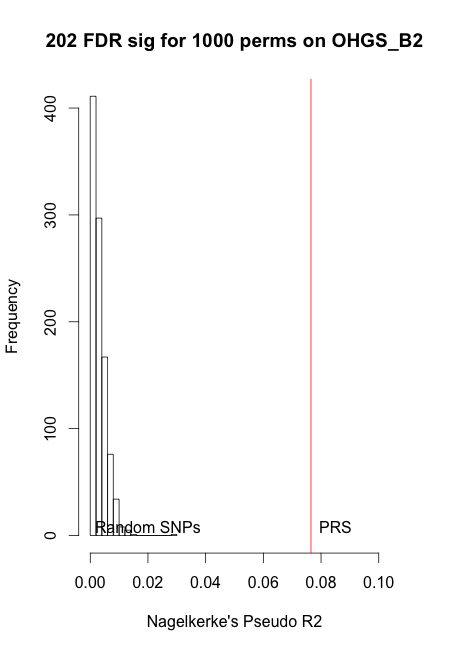
\includegraphics[width=0.5\textwidth]{Figures/b2.png}
\label{b2_perm}
\caption[$\hat{S}_{TRS}$ predicts \ac{CAD} significantly better than 1000 \ac{PRS} constructed with an equal number of \acp{SNP}.]{\textbf{$\hat{S}_{TRS}$ predicts \ac{CAD} significantly better than 1000 \ac{PRS} constructed with an equal number of \acp{SNP}.} 202 \acp{SNP} were randomly selected from post quality control imputed \acp{SNP} and a \ac{PRS} was constructed using summary information from \cite{TheCARDIoGRAMplusC4DConsortium2015} and Nagelkerke's Pseudo $R^2$ was plotted against frequency. The red line denote the Nagelkerke's $R^2$ of the true \ac{TRS} which predicts significantly $P \approx 0$ better than the random model.}
\end{figure}

These results are in line with literature values. Those in the top quintile of the \ac{PRS} were 70\% more likely to have \ac{CAD} than not (2045 cases vs 1198 controls). Similarly, those in the bottom quintile were  5\% less likely to be diagnosed with \ac{CAD} than not (1576 cases vs 1659 controls).



\section{Cardiometabolic Risk Score}

We add in each co-morbid score in a stepwise manner. $\hat{S}_{CMB; 1}$ uses just the information available for CAD and is equivalent to the above section.  $\hat{S}_{CMB; 2}$ uses information from CAD and BMI, while $\hat{S}_{CMB; 3}$ uses CAD, BMI, and LDLc. $\hat{S}_{CMB; 4}$ uses information from CAD, BMI, LDLc, and TG, while $\hat{S}_{CMB; 5}$ uses CAD, BMI, LDLc, TG, and HDLc. Note that in this section we restrict our analysis to the \ac{OHGS} cohorts along with Cleveland Clinic due to the lack of quality in lipid data present in the other cohorts. 

The summary statistics of this analysis are presented in Table \ref{cmd-sum}. Higher genetic risk scores were uniformly and significantly ($P < 2.2 \times 10^{-16}$) associated with increased risk of \ac{CAD}.

\begin{table}[H]
\centering
\begin{tabular}{lllllll}
\hline
Score & Cohort           & OR        & SE       & R2         & AIC      & AUC       \\ \hline
$\hat{S}_{CMB; 1}$     & OHGS A2          & 310.498 & 34.527 & 0.077 & 2558.277 & 0.639 \\
      & OHGS B2          & 259.593 & 24.945 & 0.074 & 3681.768 & 0.634 \\
      & OHGS C2          & 276.967 & 45.920 & 0.055 & 1318.919 & 0.619 \\
      & Cleveland Clinic & 153.899 & 36.428 & 0.017 & 1877.724 & 0.574 \\ \hline
$\hat{S}_{CMB; 2}$     & OHGS\_A2         & 252.964  & 25.292 & 0.091 & 2547.617 & 0.656 \\
      & OHGS\_B2         & 267.348   & 22.487 & 0.092 & 3654.756 & 0.650 \\
      & OHGS\_C2         & 280.924  & 38.981 & 0.077 & 1300.585 & 0.646 \\
      & Cleveland        & 337.371  & 35.182 & 0.084 & 1791.596 & 0.666 \\ \hline
$\hat{S}_{CMB; 3}$     & OHGS\_A2         & 236.0145  & 26.173 & 0.077 & 2570.063 & 0.643 \\
      & OHGS\_B2         & 255.740  & 24.099 & 0.077  & 3688.513 & 0.637 \\
      & OHGS\_C2         & 284.979  & 41.161 & 0.071 & 1305.337 & 0.640  \\
      & Cleveland        & 344.918  & 37.879 & 0.076 & 1802.024 & 0.655 \\ \hline
$\hat{S}_{CMB; 4}$     & OHGS\_A2         & 266.505  & 29.249 & 0.078 & 2568.062 & 0.644 \\
      & OHGS\_B2         & 270.889  & 26.455 & 0.073 & 3697.51  & 0.633 \\
      & OHGS\_C2         & 298.983  & 44.838 & 0.066 & 1309.38  & 0.634 \\
      & Cleveland        & 372.189   & 41.802 & 0.072 & 1806.542 & 0.651 \\ \hline
$\hat{S}_{CMB; 5}$     & OHGS\_A2         & 297.017  & 34.105 & 0.072 & 2576.54  & 0.640 \\
      & OHGS\_B2         & 299.070  & 30.767 & 0.067 & 3709.488 & 0.628 \\
      & OHGS\_C2         & 323.917  & 50.903 & 0.061 & 1313.958 & 0.628 \\
      & Cleveland        & 410.996  & 48.574 & 0.065 & 1815.742 & 0.644 \\ \hline
\end{tabular}
\label{cmd-sum}
\caption[Summary statistics from Logistic association model for $\hat{S}_{CMD}$.]{\textbf{Summary statistics from Logistic association model.} $\hat{S}_{CMD; x}$ along with the first two principal components to adjust for population stratification were used to predict \ac{CAD}. OR corresponds to the odds ratio of $\hat{S}_{TRS}$ along with its standard error (SE). $R^2$ corresponds to NagelKerke's Pseudo-$R^2$, while AIC corresponds to Akaike Information Criterion, a measure of model fit. AUC corresponds to the area under the \ac{ROC} curve as derived in the pROC package in R.}
\end{table}

In permutation analyses, each of the scores performed significantly better than an equivalent number of randomly selected \acp{SNP} in 1000 bootstraps. The random effects meta analysis \ac{AUC} values were $0.65 [ 0.64, 0.67], 0.64[0.63, 0.66], 0.64[0.63, 0.65], 0.63[0.62, 0.65]$ for scores 1 through 5 respectively. Interestingly, the more \acp{SNP} added in, the worse the model was at predicting the phenotype. The \ac{AIC} is also uniformly smaller in score 2 than in subsequent scores, meaning that this model fit the data the best. Persons in the upper quintile of this score were 81\% more likely (1725 cases vs 953 controls) to have \ac{CAD} than not (compared to 70 \% for the previous score) and people in the bottom quintile were 15.7\% less likely (1240 cases vs 1471 controls) to have \ac{CAD} than having it. There was also a substantive increase in NagelKerke's Pseudo $R^2$ in the second score compared to any other, especially in the Cleveland cohort. 

The score maintained its significance even after inclusion of biologically relevant covariates such as gender and smoking status. Additionally, the predictive accuracy of the score increased substantially after the inclusion of these covariates. After inclusion of individual's sex, a known cardiovascular risk factor, predictive accuracy increased substantially. The random effects meta analysis \ac{AUC} values were increased to $0.69[0.62, 0.76], 0.74[0.67, 0.81], 0.73 [0.66, 0.81], 0.73[0.66, 0.81], 0.73[0.66, 0.80]$ for $\hat{S}_{CMB; 1}$ through $\hat{S}_{CMB; 5}$ respectively. Again it appears as though $\hat{S}_{CMB; 2}$ is the best predictive model.


We additionally investigated whether sex significantly modulates the effect of  $\hat{S}_{CMB; .}$ and found no significant interactions. 

\subsection{Optimal Cardiometabolic Risk Score}

When optimal scores were derived, the thresholds described in Table \ref{oprs} were observed.

\begin{table}[H]
\centering

\begin{tabular}{lllll}
\hline
                  & \textbf{LDLc} & \textbf{HDLc} & \textbf{TG} & \textbf{BMI} \\ \hline
OHGS\_A2 & 0.0001        & 0.0055        & 0.1743      & 1            \\
OHGS\_B2 & 0.2484        & 0.0999        & 0.0002      & 1            \\
OHGS\_C2 & 0.1299        & 0.0085        & 0.1528      & 1            \\
CCGB\_2  & 0.1807        & 0.2039        & 0.004       & 1            \\ \hline
\end{tabular}

\caption[Optimal \ac{PRS} $P$-value thresholds.]{\textbf{Optimal \ac{PRS} $P$ value thresholds ($T_o$) derived for each trait in each cohort.} 2500 thresholds were created between $P = 0.0001$ and $P = 0.25$ and used as inclusion threshold $T$ for \ac{PRS}. These \acp{SNP} were used to construct a \ac{PRS}, which was used alongside the first two principal components and sex as covariates to predict \ac{CAD}. Their respective $P$-values of association were recorded and the maximal $-\log_{10} P$-value of association was used as the optimal threshold $T_0$.}
\label{oprs}
\end{table}


The optimal $P$ value cutoff threshold $T_o$ for \ac{BMI} was found to be $1$ for all cases as demonstrated in \ref{oprs_bmi}. We discuss this result further below, however, for now we exclude \ac{BMI} from the analysis of optimal risk scores, and opt to use just scores for the lipid traits.

\begin{figure}[H]
\centering
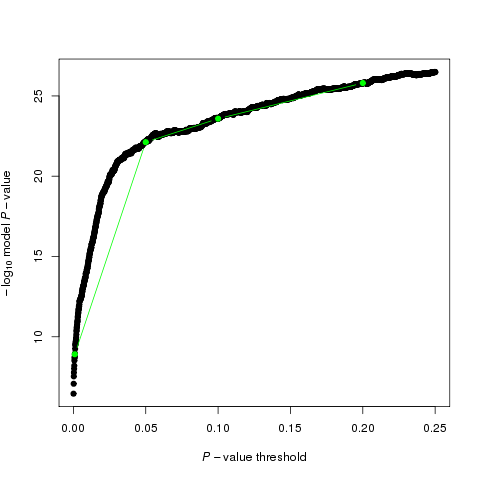
\includegraphics[width=0.5\textwidth]{Figures/PRSice_HIGH-RES_PLOT_2016-04-23.png}
\label{oprs_bmi}
\caption[Optimal $P$-value inclusion threshold for \ac{BMI}.]{\textbf{High definition assocaition plot for \ac{BMI} \acp{SNP} with \ac{CAD}.}2500 thresholds were created between $P = 0.0001$ and $P = 0.25$ and used as inclusion threshold $T$ for \ac{PRS}. These \acp{SNP} were used to construct a \ac{PRS}, which was used alongside the first two principal components and sex as covariates to predict \ac{CAD}. Their respective $P$-values of association were recorded and the maximal $-\log_{10} P$-value of association was used as the optimal threshold $T_0$. There was no maximal $-\log_{10} P$ value threshold less than 0.25, consistent with the model shown in figure \ref{pi0} with low $\pi_0$, or proportion of truly null \acp{SNP}.}
\end{figure}

Constructing a logistic regression model, we find that our cumulative score (combining optimal scores from all three traits) is significantly ($P < 2.2 \times 10^{-16}$.) associated with \ac{CAD} status, and those who have a higher \ac{PRS} tend to have higher risk for \ac{CAD}. We detail summary statistics for this association in table \ref{oprs_ss}. 



\begin{table}[H]
\centering

\begin{tabular}{lllllll}
\hline
Study & $n_{SNPs}$ & OR         & SE      & $R^2$     & AIC     & ROC    \\ \hline
OHGS\_A2 & 439971 & $2.2\times10^4$  & $1.3\times10^3$ & 0.245 & 2313    & 0.748 \\
OHGS\_B2 & 790128 & $3.42\times10^4$ & $1.5\times10^3$ & 0.338 & 3061.9  & 0.796 \\
OHGS\_C2 & 622050 & $3.34\times10^4$ & $2.5\times10^3$ & 0.301 & 1095.1  & 0.793 \\
CCGB\_2 & 847335 & $3.78\times10^4$ & $2.3\times10^3$ & 0.284 & 1517.21 & 0.795 \\ \hline
\end{tabular}
\label{oprs_ss}
\caption[Summary statistics from Logistic association model for $\hat{S}_{oCMD}$.]{\textbf{Summary statistics from Logistic association model.} $\hat{S}_{oCMD}$ along with the first two principal components to adjust for population stratification were used to predict \ac{CAD}. OR corresponds to the odds ratio of $\hat{S}_{TRS}$ along with its standard error (SE). $R^2$ corresponds to NagelKerke's Pseudo-$R^2$, while AIC corresponds to Akaike Information Criterion, a measure of model fit. AUC corresponds to the area under the \ac{ROC} curve as derived in the pROC package in R.}
\end{table}

The \ac{oPRS}, comprising optimal scores for \ac{LDLc}, \ac{HDLc}, and \ac{TG} predicts \ac{CAD} with a very high accuracy, explaining between 24.5 and 33.8 percent of variance in \ac{CAD}. The random effects meta analysis of \ac{AUC} of the \ac{ROC} curve reveals an overall \ac{AUC} of $0.78 [0.75, 0.81]$, an extremely high value (Figure \ref{oprs_meta}). 

\begin{figure}[H]
\label{oprs_meta}
\caption{Random effects meta analysis of \ac{oPRS} predicting risk for \ac{CAD}}
\centering
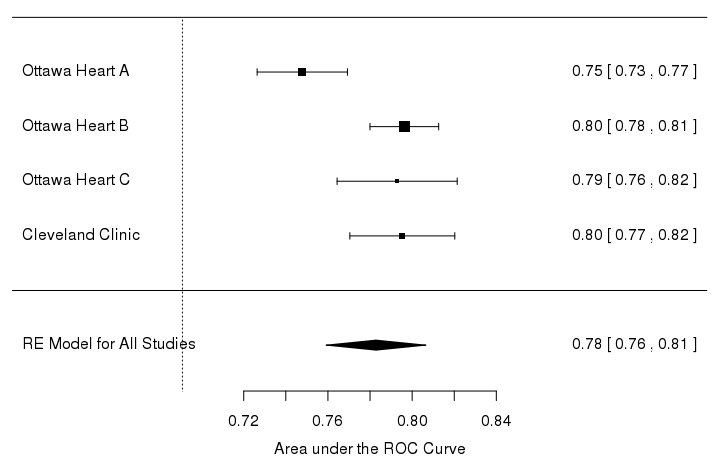
\includegraphics[width=0.5\textwidth]{Figures/oprs_meta.png}
\end{figure}


Though the \ac{AUC} varies significantly between the cohorts, it is significantly higher than any observed in either the \ac{TRS} or the \ac{CMB} scores. However, as noted in table \ref{oprs_ss}, each \ac{oPRS} comprises several hundred thousand \acp{SNP}, and it is difficult to assess whether the increase in predictive accuracy is simply a consequence of increasing the number of \acp{SNP} used to predict the phenotype, or whether it is a true biological occurrence. When an equal number of \acp{SNP} were selected at random in 1000 bootstraps, it was found that the $R^2$ of our \ac{oPRS} was not significantly $P > 0.05$ different than that obtained through permutation.


\subsection{Model Comparisons}

When the cardiometabolic $\hat{S}_{CMB; 2}$, determined to be the best predictive candidate score for \ac{CAD} was compared against the \ac{TRS} score in 1000 random bootstraps in all cohorts combined, it was found to have a significantly larger \ac{AUC} ($P < 2.2 \times 10^{-16}$). A similar result was found when the \ac{oPRS} was compared to both the \ac{TRS} and the \ac{CMB} scores. % Include the second content chapter
\chapter{Discussion}

In this thesis we have introduced a novel method for using summary information from co-morbid conditions identified through \ac{GWAS} for the prediction of complex disease. We validate this technique in a meta analysis of four cohorts.

Previously, polygenic risk scores (\ac{PRS}) have been used to predict complex diseases and to measure to genetic overlap between conditions. However, often researchers restrict themselves to using the loci which have the highest confidence -- those which reach genome-wide significance. Theoretical work disputes this notation, indicating that many low or modest effect variants may be hidden in the region of $P$-values classically called non-significant. To help better identify candidate variants which may be useful in predicting a condition, we use variants shown to be linked to co-morbid conditions in order to construct a cardiometabolic risk score for coronary artery disease (\ac{CAD}).

We use meta data from the recent large scale meta-analysis conducted by the \ac{CARDIOGRAMC4D} consortium to construct the ``traditional'' \ac{PRS} for \ac{CAD} in our four cohorts. The score performs as is expected, significantly predicting \ac{CAD} with a relatively low explained variance, with NagelKereke's Pseudo-$R^2$ averaging 4.7\% between the cohorts. This model performs decently at predicting \ac{CAD} as well, with a meta analyzed overall \ac{AUC} of the \ac{ROC} curve of 0.61 with 95\% confidence interval between 0.58 and 0.63. Adding biologically relevant covariates increases the predictive accuracy whilst the \ac{PRS} maintains its significance.  Our new model, adding together the \ac{PRS} from co-morbid conditions as in Section \ref{cmb-rs}, showed an improvement over the traditional model in all cases. However, the largest (and only statistically significant) difference occurs between the traditional risk score and the score incorporating BMI loci. Interestingly, though the subsequent scores contain all \acp{SNP} present in the second BMI score, the increased noise makes the improvement over the \ac{TRS} less pronounced. This is directly conflicting with the notion that increasing the number of \acp{SNP} used to construct the \ac{PRS} will usually increase the predictive accuracy, even if it does not increase the significance of the model.

We additionally showed that though our method involves additional \acp{SNP} to the \ac{PRS}, the increase in predictive accuracy occurs that which would be expected by chance, as shown in figure \ref{b2_perm}. This was not the case with the optimal model, as will be described below. 

We can only speculate on the true reasons for the observed pattern in \ac{PRS} association. \ac{LDLc}, \ac{HDLc}, and \ac{TG} are well known risk factors for \ac{CAD}, and perhaps these results shed some light on the underlying relationship between these phenotypes and \ac{CAD}. It has been well documented that \ac{CAD} and \ac{BMI} share a substantial genetic relationship: in a recent study, the $r_G$, or genetic correction, between these two phenotypes was estimated to be $r_G = 0.66$ with standard error $0.2$, $P = 5 \times 10^{-4}$. \citep{Cole2015a} Full results for our cohorts are displayed in table \ref{rg}. 

\begin{table}[H]
\centering
\caption{Genetic Correlations between Obesity and \ac{CAD}. Adapted from \cite{Cole2015a}}
\label{rg}
\begin{tabular}{llll}
\hline
\textbf{Study} & \textbf{Sample Size} & \textbf{$r_G$} & \textbf{SE} \\ \hline
OHGS\_A2       & 3578                 & 0.566          & 0.244       \\
OHGS\_B2       & 5718                 & 1.00           & 0.787       \\
OHGS\_C2       & 2816                 & 0.778          & 0.713       \\
CCGB\_2        & 4365                 & 0.868          & 0.496       \\ \hline
\end{tabular}
\end{table}

It is evident that \ac{BMI} and \ac{CAD} share substantial genetic pleiotropy. Similar analyses for \ac{LDLc}, \ac{HDLc}, and \ac{TG} have not been conducted. It has recently been demonstrated that adiposity, that is, \ac{BMI} \textit{per se}, significantly interacted with a \ac{PRS} for dyslpidemia. \citep{Cole2014} This adds to a body of evidence suggesting multiple gene by environment interactions may play crucial roles in dyslipidemia risk. \cite{ColeChristopherB.a;NikpayMajidb;McPhersonRutha} Thus, it remains an open question whether the genetic predisposition to \ac{BMI} is interacting with the genetic predisposition to lipids such that the results observed are unexpected.

The combined optimal model was shown to be highly effective at predicting \ac{CAD}, explaining between 24.5 and 33.8 percent of variance in the phenotype. Recall that estimated heritability $h^2$ is approximately 40\%, meaning that our score explains between 60\% and 80\% of the variance in \ac{CAD} attributable to genetics. However, it was found that predictive accuracy explained by the score may be attributable to the number of \acp{SNP} which were used in its construction, as the NagelKerke's Pseudo-$R^2$ was insignificantly different than 1000 bootstrap permutations using the same number of \acp{SNP}. Though it performed well, it is difficult to compare because of this reason. 

Additionally, we observed that the optimal solution for \ac{BMI} was trivial; that is, no $P$-value threshold $T_o <1$ was optimal. Referring to Figure \ref{pi0}, this may lend evidence to the assertion to that there is a relatively large number of small effect size \acp{SNP} influence \ac{BMI} rather than a smaller set of large effect size \acp{SNP}. This would correspond to a lower $\pi_0$, or proportion of true null \acp{SNP} and no maxima $< 1$ for $P \in [0,1]$.

Because of this, it is difficult to compare the \ac{oPRS} to either the \ac{TRS} or the \ac{CMB} scores. 

\section{Future Directions} 

Our study has provided a solid foundation upon which to further elucidate the roll which polygenic risk scores may play in both the prediction and understanding of \ac{CAD}. Future research may examine the exact algorithm by which the cardiometabolic score is calculated. Specifically, the roll and weighting of duplicated variants must be investigated to see if predictive variants which occur in more than one \ac{PRS} should be upweighted or prioritized to better facilitate phenotype prediction. Additionally, the roll of variant independence must be examined in depth; currently the optimal score does not include any reservations about variant dependency conditions. Whether or not this has impacted the predictive accuracy remains to be seen.

Additionally, the trends observed must be validated mathematically; we are unsure of the exact mechanics and expected outcomes when scores are combined such as we have done. More research must be done to better understand the benefits and drawbacks of combining information in this way.  % Include the third content chapter
\chapter{Conclusions}

In this thesis submitted to partially fulfill the requirements of an honours undergraduate degree in biomedical science, we introduce and validate a novel methodology for combining summary information from \ac{GWAS} in order to better predict complex disease from co-morbid conditions and phenotypes. We introduce \ac{GWAS} and their statistical properties, leading into a discussion of \ac{PRS}. We build upon these definitions to create our new model, which combines scores across several conditions. We find that our new \ac{CMB} score predicted \ac{CAD} significantly better than did the \ac{TRS}. We additionally constructed an optimal \ac{PRS} (\ac{oPRS}), which predicted between 60 and 80 \% of the variance in \ac{CAD} attributable to genetics, but was not significantly different from a random bootstrap. We have also shown that the characteristics of \ac{oPRS} $P$ value threshold selection in \ac{BMI} are consistent with those observed when a relatively high number of low effect \acp{SNP} affect the phenotype, lending evidence to this notion. 

Our novel scoring technique represents a significant improvement over the traditional polygeneic prediction of \ac{CAD}. However, much theoretical research is needed to validate and explore the trends observed. We believe that by pushing further into this area of knowledge, eventually \ac{PRS}, a widely used but often naive methodology, will be improved to the point of clinical utility. Using further iterations of methods like ours, eventually clinicians may be able to predict patient's clinical phenotypes with a high degree of accuracy from a small number of \acp{SNP}.


\backmatter

\chapterstyle{default} % Reset the chapter style back to the default used for non-content chapters

%----------------------------------------------------------------------------------------
%	BIBLIOGRAPHY
%----------------------------------------------------------------------------------------

\bibliographystyle{plainnat} % Use the plainnat bibliography style

\bibliography{bibliography} % Use the bibliography.bib file as the source of references

%----------------------------------------------------------------------------------------
%	INDEX
%----------------------------------------------------------------------------------------

\printindex % Print the index

%----------------------------------------------------------------------------------------

\end{document}